\section{História}

\begin{frame}
	\frametitle{Curiosidade}
	\begin{figure}[htpb]
		\centering
		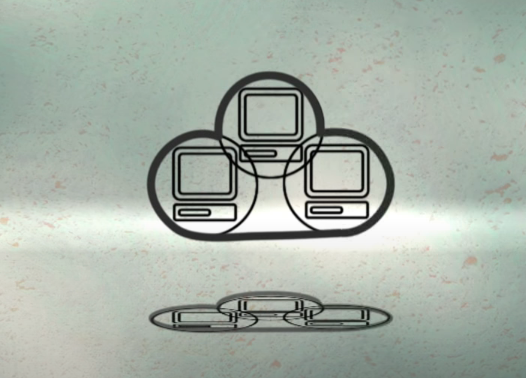
\includegraphics[width=0.6\textwidth]{server_cluster}
		\caption{A cluster of servers drawn in a system diagram \footnote{\href{https://www.youtube.com/watch?v=e3UMvBP2RRo}{Image source link}}}
	\end{figure}
\end{frame}

\subsection{Linha do tempo}

\begin{frame}
	\frametitle{Linha do tempo}
	\begin{center}
		História da computação em nuvem\cite{CCHistory}
	\end{center}
	\hfill
	\begin{scriptsize}
	\begin{bf}
	\begin{center}
		\begin{chronology}[10]{1955}{2010}{12cm}[\textwidth]
			\event[1955]{1965}{1955-1965}
			\event[1970]{1990}{1970-1990}
			\event[1990]{2006}{1990-2006}
			\event{2006}{2006}
			\event[2006]{2010}{2016-2010}
		\end{chronology}
	\end{center}
	\end{bf}
	\hfill
	\begin{itemize}
		\item (1955-1965) Problemas na infraestrutura de TI
		\item (1970-1990) Hypervisors e a internet
		\item (1990-2006) Internet para todos
		\item (2006-2006) Precipitation
		\item (2006-2010) Primeiros dias da computação em nuvem
	\end{itemize}
	\end{scriptsize}
\end{frame}

\begin{frame}
	\frametitle{Linha do tempo}
	\begin{center}
		Problemas na infraestrutura de TI \\ (1955-1965)
	\end{center}
	\hfill
	\begin{scriptsize}
	\begin{bf}
	\begin{center}
		\begin{chronology}[10]{1955}{2010}{12cm}[\textwidth]
			\event[1955]{1965}{1955-1965}
			\event[1970]{1990}{1970-1990}
			\event[1990]{2006}{1990-2006}
			\event{2006}{2006}
			\event[2006]{2010}{2016-2010}
			\color{lightgreen}
				\event[1955]{1965}{1955-1965}
		\end{chronology}
	\end{center}
	\end{bf}
	\end{scriptsize}
\end{frame}

\begin{frame}[allowframebreaks]
	\frametitle{(1955-1965) Problemas na infraestrutura de TI}
	\begin{itemize}
		\item 1942 - John Vincent Atanasoff construiu o computador ABC
		\item Server/Mainframe (Componentes principais):
			\begin{itemize}
				\item Uma CPU
				\item Um dispositivo de armazenamento de dados
			\end{itemize}
		\item 1960 - Muito caro para aderir os computadores
			\begin{itemize}
				\item Sala inteira para o servidor (Manter temperatura ideal, espaço, etc\dots)
				\item Computador
				\item Funcionários especializados
				\item Problemas para adaptar o software
			\end{itemize}
		\item Apenas empresas que com poder aquisitivo conseguiram aderir os computadores
		\item 1961 - John MacCharty fez uma palestra no MIT
			\begin{itemize}
				\item Computação poderia ser vendida como água ou eletricidade \cite{SimsonTCI}
				\item Mas seria necessário de uma grande evolução tecnológica
			\end{itemize}
	\end{itemize}
\end{frame}

\begin{frame}
	\frametitle{Linha do tempo}
	\begin{center}
		Hypervisors e a internet \\
		(1970-1990)
	\end{center}
	\hfill
	\begin{scriptsize}
	\begin{bf}
	\begin{center}
		\begin{chronology}[10]{1955}{2010}{12cm}[\textwidth]
			\event[1955]{1965}{1955-1965} \event[1970]{1990}{1970-1990}
			\event[1990]{2006}{1990-2006}
			\event{2006}{2006}
			\event[2006]{2010}{2016-2010}
			\color{lightgreen}
				\event[1970]{1990}{1970-1990}
		\end{chronology}
	\end{center}
	\end{bf}
	\end{scriptsize}
\end{frame}

\begin{frame}[allowframebreaks]
	\frametitle{(1970-1990) Hypervisors e a internet}
	\begin{itemize}
		\item Diminiur os custos da adoção do computador
			\begin{itemize}
				\item Múltiplos usuários podem compartilhar o mesmo armazenamento e o poder de processamento da CPU
			\end{itemize}
		\item 1970 - Nasceu a tecnologia da virtualização
			\begin{itemize}
				\item Um computador pode ser particionado em vários partes
				\item Cada parte pode rodar um código independente
				\item Cada parte é chamada de Máquina Virtual (VM)
				\item O server principal é chamado de \it{host}
			\end{itemize}
		\item 1983 - A internet nasceu
			\begin{itemize}
				\item Começou pelo projeto ARPANet para comunicação de professores de universidades
			\end{itemize}
		\item Foi introduzida a arquitetura cliente-servidor, o cliente e o server eram os mainframes interagindo com código e informação conectados por cabos (Internet)
		\item Conforme os números de páginas foram crescendo o número de servers cresceram
			\begin{itemize}
				\item Os servers se moveram para datacenters
			\end{itemize}
	\end{itemize}
\end{frame}

\begin{frame}
	\frametitle{Linha do tempo}
	\begin{center}
		Internet para todos \\
		(1990-2006)
	\end{center}
	\hfill
	\begin{scriptsize}
	\begin{bf}
	\begin{center}
		\begin{chronology}[10]{1955}{2010}{12cm}[\textwidth]
			\event[1955]{1965}{1955-1965}
			\event[1970]{1990}{1970-1990}
			\event[1990]{2006}{1990-2006}
			\event{2006}{2006}
			\event[2006]{2010}{2016-2010}
			\color{lightgreen}
				\event[1990]{2006}{1990-2006}
		\end{chronology}
	\end{center}
	\end{bf}
	\end{scriptsize}
\end{frame}

\begin{frame}[allowframebreaks]
	\frametitle{(1990-2006) Internet para todos}
	\begin{itemize}
		\item A empresas maiores precisavam de datacenters maiores
		\item Problemas:
			\begin{itemize}
				\item Ociosidade quando seu website não está sendo acessado. Trazendo prejuízo para as empresas com os servers ativos
				\item A escalabilidade era feita de forma manual e precisava de dispositivos físicos. Seria muito difícil acompanhar o crescimento da aplicação
				\item As atualizações eram feitas manualmente, e precisariam possívelmente consertar as máquinas. Perdendo um tempo precioso
				\item A experiência do usuário não era boa. A distância do server impacta o delay da página
			\end{itemize}
	\end{itemize}
\end{frame}

\begin{frame}
	\frametitle{Linha do tempo}
	\begin{center}
		Precipitation \\
		(2006)
	\end{center}
	\hfill
	\begin{scriptsize}
	\begin{bf}
	\begin{center}
		\begin{chronology}[10]{1955}{2010}{12cm}[\textwidth]
			\event[1955]{1965}{1955-1965}
			\event[1970]{1990}{1970-1990}
			\event[1990]{2006}{1990-2006}
			\event{2006}{2006}
			\event[2006]{2010}{2016-2010}
			\color{lightgreen}
				\event{2006}{2006}
		\end{chronology}
	\end{center}
	\end{bf}
	\end{scriptsize}
\end{frame}

\begin{frame}[allowframebreaks]
	\frametitle{(2006) Precipitação}
	\begin{itemize}
		\item Grandes empresas (\it{Google, Amazon, eBay, etc\dots})
			\begin{itemize}
				\item Criaram \it{data centers} com centenas/milhares de servers de alta qualidade no mundo inteiro
				\item Por causa dos prejuízos decidiram começar a alugar essas máquinas
			\end{itemize}
		\item 2006 - "Cloud Computing" foi introduzino no mundo como forma de aluguel de poder computacional
		\item A Amazon chamou essa divisão de Amazon Web Services (AWS)
		\item A AWS foi a primeira de muitos provedores de cloud
		\item Depois de 50 anos o sonho de John McCharty foi realizado
	\end{itemize}
\end{frame}

\begin{frame}
	\frametitle{Linha do tempo}
	\begin{center}
		Primeiros dias da computação em nuvem \\
		(2006-2010)
	\end{center}
	\hfill
	\begin{scriptsize}
	\begin{bf}
	\begin{center}
		\begin{chronology}[10]{1955}{2010}{12cm}[\textwidth]
			\event[1955]{1965}{1955-1965}
			\event[1970]{1990}{1970-1990}
			\event[1990]{2006}{1990-2006}
			\event{2006}{2006}
			\event[2006]{2010}{2016-2010}
			\color{lightgreen}
				\event[2006]{2010}{2016-2010}
		\end{chronology}
	\end{center}
	\end{bf}
	\end{scriptsize}
\end{frame}

\begin{frame}[allowframebreaks]
	\frametitle{(2006-2010) Primeiros dias da computação em nuvem}
	\begin{itemize}
		\item Por 6 anos a AWS estabeleceu seu monopólio na área de nuvem
		\item A computação em nuvem permitiu que as empresa pudessem dar um foco maior no desenvolvimento
			\begin{itemize}
				\item Os dados são criptografados e seguros
				\item Dados são armazenados com redundância em nuvem
				\item Escalabilidade
				\item De fácil deploy
				\item Alta disponibilidade
			\end{itemize}
	\end{itemize}
\end{frame}

\begin{frame}
	\frametitle{(2006-2010) Primeiros dias da computação em nuvem}
	\begin{figure}[htpb]
	\begin{center}
	\begin{tiny}
	\begin{tikzpicture}[scale=1, transform shape]
		\node (A) at (0,4) {\normalsize On-Site};
		\node (A1) at ($(A) - (0,0.6)$)  [draw,thick,minimum width=75,minimum height=15] {Applicação};
		\node (A2) at ($(A1) - (0,0.6)$) [draw,thick,minimum width=75,minimum height=15] {Data};
		\node (A3) at ($(A2) - (0,0.6)$) [draw,thick,minimum width=75,minimum height=15] {Runtime};
		\node (A4) at ($(A3) - (0,0.6)$) [draw,thick,minimum width=75,minimum height=15] {Middleware};
		\node (A5) at ($(A4) - (0,0.6)$) [draw,thick,minimum width=75,minimum height=15] {O/S};
		\node (A6) at ($(A5) - (0,0.6)$) [draw,thick,minimum width=75,minimum height=15] {Virtualization};
		\node (A7) at ($(A6) - (0,0.6)$) [draw,thick,minimum width=75,minimum height=15] {Servers};
		\node (A8) at ($(A7) - (0,0.6)$) [draw,thick,minimum width=75,minimum height=15] {Storage};
		\node (A9) at ($(A8) - (0,0.6)$) [draw,thick,minimum width=75,minimum height=15] {Networking};
		\node (B) at (3,4) {\normalsize IaaS};
		\node (B1) at ($(B) - (0,0.6)$)  [draw,thick,minimum width=75,minimum height=15] {Applicação};
		\node (B2) at ($(B1) - (0,0.6)$) [draw,thick,minimum width=75,minimum height=15] {Data};
		\node (B3) at ($(B2) - (0,0.6)$) [draw,thick,minimum width=75,minimum height=15] {Runtime};
		\node (B4) at ($(B3) - (0,0.6)$) [draw,thick,minimum width=75,minimum height=15] {Middleware};
		\node (B5) at ($(B4) - (0,0.6)$) [draw,thick,minimum width=75,minimum height=15] {O/S};
		\node (B6) at ($(B5) - (0,0.6)$) [lightgreen,draw,thick,minimum width=75,minimum height=15] {Virtualization};
		\node (B7) at ($(B6) - (0,0.6)$) [lightgreen,draw,thick,minimum width=75,minimum height=15] {Servers};
		\node (B8) at ($(B7) - (0,0.6)$) [lightgreen,draw,thick,minimum width=75,minimum height=15] {Storage};
		\node (B9) at ($(B8) - (0,0.6)$) [lightgreen,draw,thick,minimum width=75,minimum height=15] {Networking};
		\node (C) at (6,4) {\normalsize PaaS};
		\node (C1) at ($(C) - (0,0.6)$)  [draw,thick,minimum width=75,minimum height=15] {Applicação};
		\node (C2) at ($(C1) - (0,0.6)$) [draw,thick,minimum width=75,minimum height=15] {Data};
		\node (C3) at ($(C2) - (0,0.6)$) [lightgreen,draw,thick,minimum width=75,minimum height=15] {Runtime};
		\node (C4) at ($(C3) - (0,0.6)$) [lightgreen,draw,thick,minimum width=75,minimum height=15] {Middleware};
		\node (C5) at ($(C4) - (0,0.6)$) [lightgreen,draw,thick,minimum width=75,minimum height=15] {O/S};
		\node (C6) at ($(C5) - (0,0.6)$) [lightgreen,draw,thick,minimum width=75,minimum height=15] {Virtualization};
		\node (C7) at ($(C6) - (0,0.6)$) [lightgreen,draw,thick,minimum width=75,minimum height=15] {Servers};
		\node (C8) at ($(C7) - (0,0.6)$) [lightgreen,draw,thick,minimum width=75,minimum height=15] {Storage};
		\node (C9) at ($(C8) - (0,0.6)$) [lightgreen,draw,thick,minimum width=75,minimum height=15] {Networking};
		\node (D) at (9,4) {\normalsize SaaS};
		\node (D1) at ($(D) - (0,0.6)$)  [lightgreen,draw,thick,minimum width=75,minimum height=15] {Applicação};
		\node (D2) at ($(D1) - (0,0.6)$) [lightgreen,draw,thick,minimum width=75,minimum height=15] {Data};
		\node (D3) at ($(D2) - (0,0.6)$) [lightgreen,draw,thick,minimum width=75,minimum height=15] {Runtime};
		\node (D4) at ($(D3) - (0,0.6)$) [lightgreen,draw,thick,minimum width=75,minimum height=15] {Middleware};
		\node (D5) at ($(D4) - (0,0.6)$) [lightgreen,draw,thick,minimum width=75,minimum height=15] {O/S};
		\node (D6) at ($(D5) - (0,0.6)$) [lightgreen,draw,thick,minimum width=75,minimum height=15] {Virtualization};
		\node (D7) at ($(D6) - (0,0.6)$) [lightgreen,draw,thick,minimum width=75,minimum height=15] {Servers};
		\node (D8) at ($(D7) - (0,0.6)$) [lightgreen,draw,thick,minimum width=75,minimum height=15] {Storage};
		\node (D9) at ($(D8) - (0,0.6)$) [lightgreen,draw,thick,minimum width=75,minimum height=15] {Networking};
	\end{tikzpicture}
	\end{tiny}
	\end{center}
	\caption{Imagem retirado do site da redhat\footnote{\href{https://www.redhat.com/cms/managed-files/iaas-paas-saas-diagram5.1-1638x1046.png}{RedHat IaaS, PaaS e SaaS}}}
	\end{figure}
\end{frame}
